\chapter{Regionenbasiertes Matching}
Die vorab beschriebenen Parameter der Bildaufteilung flie\ss en nun in den Matchingprozess mit ein und sollen dazu verwendet werden, fehlerhafte Matches zu filtern.

%CITE

\section{Regionierung des Datensatzes}
Ein Begriff der die Isolation eines Bereiches innerhalb eines Bildes beschreibt und eng mit der Bedeutung der Segmentierung und Klassifikation zusammenh\"angt. Dabei werden hier, anhand von Vorwissen, Bildregionen mit zus\"atzlichen Informationen bez\"uglich ihrer geometrischen Lage versehen. Das Unterteilen eines Bildes in verschiedene Bereiche impliziert zun\"achst die Funktionalit\"at eine Region zu definieren, die eine Teilmenge aller Bildpunkte enth\"alt. \"Uber diese Masken l\"asst sich im Folgenden leicht bestimmen, ob sich ein Bildpunkt innerhalb oder au\ss erhalb dieser befindet. Die Form einer Region wird dabei \"uber die manuell gesetzten Eckpunkte und der dadurch eingeschlossenen Fl\"ache festgelegt.\\
Als angepasster Ansatz wurde sich f\"ur eine polygone Regionsabgrenzung der unterschiedlichen Fassaden entschieden, wobei theoretisch Vierecke gen\"ugen w\"urden. Jedoch lassen sich durch eine polygone Fl\"ache m\"uhelos Verdeckungen, wie andere Bauwerke oder Vegetation, innerhalb der Fotos umgehen, die jene Au\ss enseiten des AfE-Turms bedecken.

\begin{figure}[h]
\centering
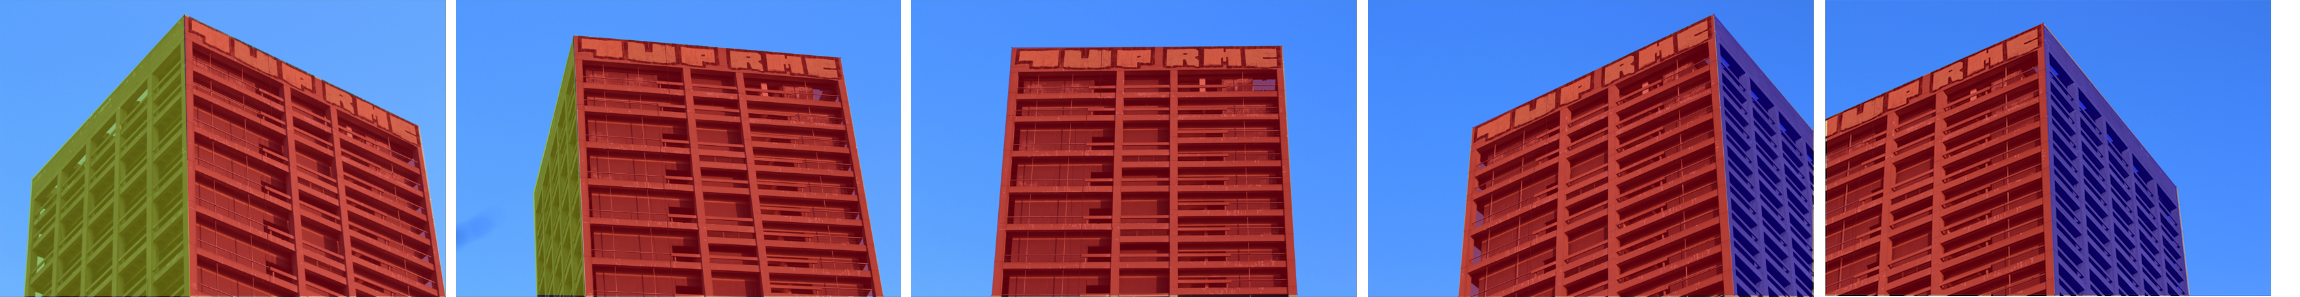
\includegraphics[width=0.9\textwidth]{gfx/regreihe.png}
\caption[F\"unf regionierte Bilder des AfE-Turms]{F\"unf regionierte Bilder des AfE-Turms}
\label{gr:afeturmreg}
\end{figure}
\FloatBarrier

Wichtig ist zu erw\"ahnen, dass nicht nur vorab festgelegte Regionen eines Bildes vom angepassten Matchingverfahren ber\"ucksichtigt werden, sondern auch noch immer Features aus nicht markierten Bereichen betrachtet werden. So hat jeder unterteilte Bereich eine eindeutige Identifikation, ebenso wie nicht markierte. Alle au\ss erhalb der Regionen liegende Bildpunkte werden zu einer \glqq Unknown\grqq \ Region (Regions-ID: -1) zusammengefasst. Dieser Bereich wird also wie eine Region behandelt und dessen Features werden nur mit anderen Features gematcht, die auch in dieser \glqq Unknown\grqq \ Region liegen.\\
Dieser Ansatz soll fehlerhafte Matches entfernen, jedoch zutreffende unber\"uhrt lassen.

\subsection{Schnitttest einer Region}
Um zu \"uberpr\"ufen, ob bestimmte Bildpunkte einer gewissen Region angeh\"oren, ist es f\"ur das sp\"atere Matchingverfahren n\"otig, dass vor dem Matching \"uberpr\"uft werden kann, ob ein vermeintbares Feature-Paar auch zul\"assig ist. Hierzu wird mittels Strahl-Methode des Punkt-in-Polygon-Tests nach Jordan\cite{hake1994kartographie}\cite{bartelme1995geoinformatik} \"uberpr\"uft, ob sich ein Bildpunkt innerhalb einer der Regionen befindet. Ein Polygon l\"asst sich auch als eine Menge gerichteter Liniensegmente betrachten. Bei der Strahl-Methode wird, vereinfacht gesagt, vom zu testenden Punkt aus ein Strahl in eine beliebige Richtung gesendet und die Anzahl der Schnittpunkte mit den Liniensegmente gez\"ahlt. Bei ungerader Zahl befindet sich der Punkt innerhalb des Polygons und andersherum bei gerader Anzahl au\ss erhalb. Ein gro\ss er Vorteil dieser Methode ist, dass sowohl konvexe als auch konkave Polygone gleicherma\ss en behandelt werden k\"onnen. 

\section{Das RGN-Dateiformat}
Zus\"atzlich zu den einzelnen Views, deren zugeh\"orige Parameter in einer MVE-Datei abgelegt sind, m\"ussen somit auch Informationen zu Form und Position der zugeh\"origen Regionen aufgenommen werden. Im Sinne der Wiederverwendbarkeit, wird hierf\"ur ein eigenes Dateiformat 
definiert anstatt die Regionsparameter in bereits existierende Softwareigene Dateitypen zu schreiben. Somit l\"asst sich auf jene Parameter zugreifen, auch ohne einen kompletten View zu laden.\\
Regionen werden pro View in eine RGN-Datei geschrieben. Das hier verwendete Format enth\"alt sowohl relative Positionen der Eckpunkte aller Polygone als auch deren Identifizierung und setzt sich wie folgt zusammen:


\begin{table}[h]
\begin{tabular}{|c|}
\hline
\begin{tabular}[c]{@{}c@{}}Region 1-ID\\ x-Koordinate Punkt 1\\ y-Koordinate Punkt 1\\ ...\\ x-Koordinate Punkt n\\ y-Koordinate Punkt n\end{tabular} \\ \hline
\begin{tabular}[c]{@{}c@{}}Region 2-ID\\ x-Koordinate Punkt 1\\ y-Koordinate Punkt 1\\ ...\\ x-Koordinate Punkt n\\ y-Koordinate Punkt n\end{tabular} \\ \hline
...                                                                                                                                                   \\ \hline
\begin{tabular}[c]{@{}c@{}}Region n-ID\\ x-Koordinate Punkt 1\\ y-Koordinate Punkt 1\\ ...\\ x-Koordinate Punkt n\\ y-Koordinate Punkt n\end{tabular} \\ \hline
\end{tabular}
\caption[Aufbau des RGN-Dateiformats]{Aufbau des RGN-Dateiformats}
\label{tab:rgn}
\end{table}

Falls f\"ur einen Datensatz an Fotografien f\"ur jedes Bild eine Regionierung vorgenommen wurde, existieren folglich ebenso viele RGN-Dateien wie MVE-Dateien.

\section{Matchingansatz}
Rekonstruktionen mittels Bilddaten, die ein sehr homogenes und gleichm\"a\ss ig texturiertes Modell zeigen, k\"onnen oftmals fehlschlagen, da bei der Merkmalsextraktion Korrespondenzen in Bildern erfasst werden, die tats\"achlich nicht zugeh\"orig sind.\\
Durch die Regionierung liegen nun zus\"atzliche Informationen vor mit denen \"uberpr\"uft wird, ob zwei zu testende Feature-Punkte zul\"assig sind. Genauer bedeutet das, es wird mit der zuvor beschriebenen Strahl-Methode f\"ur jedes Feature \"uberpr\"uft, ob und welcher der Regionen es zugeh\"orig ist. Somit k\"onnen vorm eigentlichen Matchingansatz schon unzutreffende Korrespondenzen ausgeschlossen werden, indem nur Elemente aus Regionen mit selber ID verglichen werden. Damit kein m\"oglicher Match ausgeschlossen wird, werden auch die nicht markierten Bildbereiche ber\"ucksichtigt und untereinander gematcht.